\section{Analysis and Results}
	This chapter of the dissertation describes the processes utilized in the analysis of data produced by the systems and procedures described in the Methodology section. Also presented is the results of said analysis, providing evidence for claims made in the Conclusion.
	
	\subsection{Statistical Analysis of Index of Performance}
		With the average \(IP\) of each group calculated, analysis and comparison of the results could  commence. Individually the \(IP\)s reveal very little of interest, thus the analysis of demographics (Dyslexic and non-Dyslexic) was conducted to determine if any obvious traits existed to aid in differentiation.
				
		\begin{table}[h]
			\centering
			\caption{Pattern 3 - Average Fitts's \(IP\) per Sector Excluding Errors}
			\label{tab_pat_3_ip}
			\begin{tabularx}{\textwidth}{|l|l|X|X|X|X|X|X|X|}
				\hline
				\multicolumn{1}{|c|}{\textbf{Status}} & \multicolumn{1}{c|}{\textbf{Hand}} & \multicolumn{1}{c|}{\textbf{1}} & \multicolumn{1}{c|}{\textbf{2}} & \multicolumn{1}{c|}{\textbf{3}} & \multicolumn{1}{c|}{\textbf{4}} & \multicolumn{1}{c|}{\textbf{5}} & \multicolumn{1}{c|}{\textbf{6}} & \multicolumn{1}{c|}{\textbf{7}} \\ \hline
				Dyslexic                              & Dominant                           & 3.21       & 4.17       & 3.77       & 3.45       & 3.61       & 3.44       & 4.03       \\ \hline
				n-Dyslexic                          & Dominant                           & 3.08       & 4.04       & 4.24       & 3.69       & 3.55       & 3.75       & 4.01       \\ \hline
				Dyslexic                              & n-Dominant                       & 3.04       & 3.50       & 4.43       & 3.34       & 3.72       & 3.79       & 4.22       \\ \hline
				n-Dyslexic                          & n-Dominant                       & 3.09       & 3.89       & 3.99       & 3.27       & 3.52       & 4.18       & 3.50       \\ \hline
			\end{tabularx}
			\end{table}
			
		\begin{table}[h]
			\centering
			\caption{Pattern 4 - Average Fitts's \(IP\) per Sector Excluding Errors}
			\label{tab_pat_4_ip}
			\begin{tabularx}{\textwidth}{|l|l|X|X|X|X|X|X|X|X|}
				\hline
				\multicolumn{1}{|c|}{\textbf{Status}} & \multicolumn{1}{c|}{\textbf{Hand}} & \multicolumn{1}{c|}{\textbf{1}} & \multicolumn{1}{c|}{\textbf{2}} & \multicolumn{1}{c|}{\textbf{3}} & \multicolumn{1}{c|}{\textbf{4}} & \multicolumn{1}{c|}{\textbf{5}} & \multicolumn{1}{c|}{\textbf{6}} & \multicolumn{1}{c|}{\textbf{7}} & \multicolumn{1}{c|}{\textbf{8}} \\ \hline
				Dyslexic                              & Dominant                           & 3.68                            & 3.71                            & 4.47                            & 3.80                            & 3.77                            & 4.03                            & 4.34                            & 3.77                            \\ \hline
				n-Dyslexic                          & Dominant                           & 4.21                            & 3.61                            & 4.06                            & 3.81                            & 3.56                            & 3.81                            & 4.05                            & 4.01                            \\ \hline
				Dyslexic                              & n-Dominant                       & 3.29                            & 3.50                            & 3.49                            & 4.57                            & 3.81                            & 3.78                            & 3.52                            & 4.21                            \\ \hline
				n-Dyslexic                          & n-Dominant                       & 3.79                            & 4.06                            & 3.70                            & 3.87                            & 3.45                            & 3.60                            & 3.30                            & 4.18                            \\ \hline
			\end{tabularx}
		\end{table}		
	
		\begin{figure}[h]
		\centering
		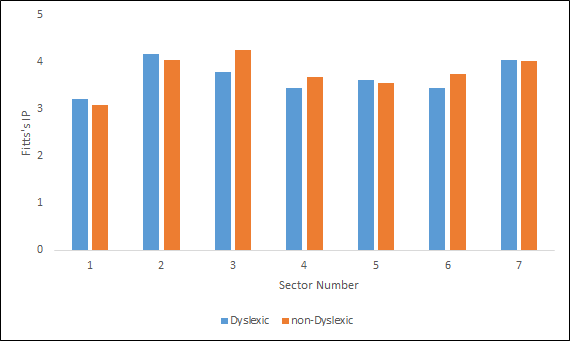
\includegraphics[width = \textwidth]{pat_3_ip_val_dom}
		\caption{Average Fitts's \(IP\) for pattern 3 sectors without errors, executed with the dominant hand.}
		\label{fig_pat_3_ip_dom}
	\end{figure}		
	
	\begin{figure}[h]
		\centering
		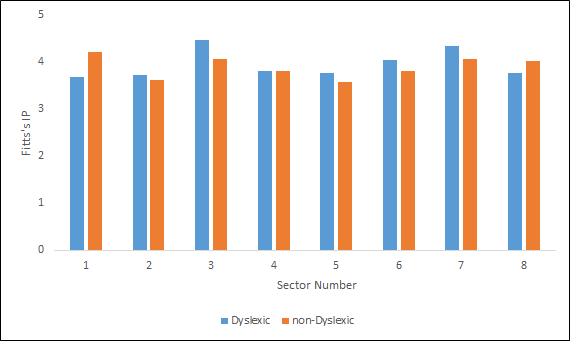
\includegraphics[width = \textwidth]{pat_4_ip_val_dom}
		\caption{Average Fitts's \(IP\) for pattern 4 sectors without errors, executed with the dominant hand.}
		\label{fig_pat_4_ip_dom}
	\end{figure}

	When comparing the average \(IP\) for Dyslexic and non-Dyslexic task participants it was found that there was very little difference between the groups (Tables \ref{tab_pat_3_ip}-\ref{tab_pat_4_ip}, Figures \ref{fig_pat_3_ip_dom}-\ref{fig_pat_4_ip_dom}, \ref{fig_pat_3_ip_ndom}-\ref{fig_pat_4_ip_ndom} ). The initial comparison was performed with the exclusion of sectors in which errors had been made. It was hypothesised that the exclusion of errors may have been the reason for the similarity in \(IP\)s, thus analysis was conducted again, this time with the inclusion of all sectors. Once again it was found that the average \(IP\)s of the Dyslexic and non-Dyslexic groups was remarkable similar, even with the inclusion of sectors with errors (Tables \ref{tab_pat_3_ip_all}-\ref{tab_pat_4_ip_all}).
	
	\begin{table}[h]
		\centering
		\caption{Pattern 3 - Average Fitts's \(IP\) per Sector Including Errors}
		\label{tab_pat_3_ip_all}
		\begin{tabularx}{\textwidth}{|r|r|X|X|X|X|X|X|X|}
			\hline
			\multicolumn{1}{|c|}{\textbf{Status}} & \multicolumn{1}{c|}{\textbf{Hand}} & \multicolumn{1}{c|}{\textbf{1}} & \multicolumn{1}{c|}{\textbf{2}} & \multicolumn{1}{c|}{\textbf{3}} & \multicolumn{1}{c|}{\textbf{4}} & \multicolumn{1}{c|}{\textbf{5}} & \multicolumn{1}{c|}{\textbf{6}} & \multicolumn{1}{c|}{\textbf{7}} \\ \hline
			Dyslexic                              & Dominant                           & 2.67       & 3.57       & 3.48       & 3.74       & 3.37       & 3.12       & 3.88       \\ \hline
			n-Dyslexic                          & Dominant                           & 2.75       & 3.61       & 3.61       & 3.62       & 3.46       & 3.18       & 3.93       \\ \hline
			Dyslexic                              & n-Dominant                       & 2.74       & 3.51       & 3.59       & 3.47       & 3.46       & 3.38       & 3.65       \\ \hline
			n-Dyslexic                          & n-Dominant                       & 2.69       & 3.24       & 3.35       & 3.30       & 3.09       & 3.11       & 3.34       \\ \hline
		\end{tabularx}
	\end{table}


	\begin{table}[h]
		\centering
		\caption{Pattern 4 - Average Fitts's \(IP\) per Sector Including Errors}
		\label{tab_pat_4_ip_all}
		\begin{tabularx}{\textwidth}{|r|r|X|X|X|X|X|X|X|X|}
			\hline
			\multicolumn{1}{|c|}{\textbf{Status}} & \multicolumn{1}{c|}{\textbf{Hand}} & \multicolumn{1}{c|}{\textbf{1}} & \multicolumn{1}{c|}{\textbf{2}} & \multicolumn{1}{c|}{\textbf{3}} & \multicolumn{1}{c|}{\textbf{4}} & \multicolumn{1}{c|}{\textbf{5}} & \multicolumn{1}{c|}{\textbf{6}} & \multicolumn{1}{c|}{\textbf{7}} & \multicolumn{1}{c|}{\textbf{8}} \\ \hline
			Dyslexic                              & Dominant                           & 2.87       & 3.51       & 3.66       & 3.56       & 3.61       & 3.96       & 3.53       & 3.67       \\ \hline
			n-Dyslexic                          & Dominant                           & 3.11       & 3.45       & 3.66       & 3.71       & 3.50       & 3.72       & 3.72       & 3.63       \\ \hline
			Dyslexic                              & n-Dominant                       & 2.97       & 3.49       & 3.33       & 3.77       & 3.57       & 3.73       & 3.19       & 3.90       \\ \hline
			n-Dyslexic                          & n-Dominant                       & 3.04       & 3.46       & 3.39       & 3.46       & 3.29       & 3.62       & 3.04       & 3.70       \\ \hline
		\end{tabularx}
	\end{table}

		While the overall averages of the populations may be similar, this does not mean that the populations are statistically similar. There exists a number of methods for the measurement of statistical similarities between populations, including t-tests, f-tests and Analysis of Variance (ANOVA).

		For the analysis of the Dyslexic and Non-Dyslexic \(IP\)s, a two sample t-test of unequal variance (sometimes referred to as a Welch test)  was chosen. The Welch test was chosen for a number of reasons, namely that only two data sets are being compared, the two data sets are completely unrelated and the number of members in each population are uneven. If comparison of the possibly Dyslexic group was also being considered then an f-test would be more appropriate. However, it is assumed that the possibly Dyslexic population consisted of a mixture of both Dyslexic and non-Dyslexic members, meaning any statistical analysis of said group would be inconclusive.

		In order to perform a proper statistical analysis, two terms had to be defined; a null hypothesis and a \(p\)-value. A null hypothesis is the formal statement of what is being tested. In the case of this project, the following null hypothesis was defined,
		‘Dyslexic and non-Dyslexic produce similar Indices of Performance for the Dot-to-Dot Task.’
		
		The p value is a pre-determined value that the result of the statistical analysis results is compared against. For the following analysis a p value of 0.05 is assumed. To summarise, if statistical analysis produces a value lesser than the p value ($\leq$ 0.05), then the null hypothesis has been disproven and is rejected. If the resulting value is greater than the p value ($\geq$ 0.05), then the null hypothesis has not been disproven. The results of the t-tests are presented in Tables \ref{tab_pat_3_t} and \ref{tab_pat_4_t}.

		\begin{table}[h]
			\centering
			\caption{Pattern 3 - t-test results.}
			\label{tab_pat_3_t}
			\begin{tabularx}{\textwidth}{|r|X|X|X|X|X|X|X|}
				\hline
				\textbf{Dominant}   & 0.7139 & 0.8733 & 0.5921 & 0.6993 & 0.6812 & 0.7923 & 0.8551 \\ \hline
				\textbf{n-Dominant} & 0.8200 & 0.2123 & 0.3265 & 0.5139 & 0.1065 & 0.2125 & 0.2227 \\ \hline
			\end{tabularx}
		\end{table}
	
		\begin{table}[h]
			\centering
			\caption{Pattern 4 - t-test results.}
			\label{tab_pat_4_t}
			\begin{tabularx}{\textwidth}{|r|X|X|X|X|X|X|X|X|}
				\hline
				\textbf{Dominant}   & 0.4200 & 0.7849 & 0.9922 & 0.5368 & 0.6723 & 0.3978 & 0.4357 & 0.8660 \\ \hline
				\textbf{n-Dominant} & 0.7545 & 0.8909 & 0.7539 & 0.1907 & 0.2545 & 0.6804 & 0.4491 & 0.4630 \\ \hline
			\end{tabularx}
		\end{table}
		
		It was found that none of the t-values for any pattern or any sector were lower than the predetermined p value. This was the case across all sectors of both pattern 3 and 4, as well as dominant and non-dominant hands. This infers that the previously stated null hypothesis is correct. 

		It should be noted that while the results of the t-test indicate that \(IP\) and thus Fitts’s Law are not a valid metric for the identification of Dyslexia, the manner of performing the analysis was atypical of the the more usual Fitts’s Analysis experiment.

	\subsubsection{Error Analysis}
		The original proposal of this project suggested that sectors in which errors occurred would be ignored. However, upon performing statistical analysis, this decision was reconsidered. During the reassessment of the inclusion of sectors with errors a trait in the data was identified. When the average number of errors for each sector in each population is considered - Dyslexic and non-Dyslexic - they appear to to be relatively similar, baring a single sector in each pattern(Tables \ref{tab_pat_3_com}-\ref{tab_pat_4_com}, Figures \ref{fig_pat_3_com_dom}-\ref{fig_pat_4_com_dom}, \ref{fig_pat_3_com_ndom}-\ref{fig_pat_4_com_ndom}).
					
		\begin{table}[h]
			\centering
			\caption{Pattern 3 - Average sector completion rate with no errors.}
			\label{tab_pat_3_com}
			\begin{tabularx}{\textwidth}{|r|r|X|X|X|X|X|X|X|}
				\hline
				\multicolumn{1}{|c|}{\textbf{Status}} & \multicolumn{1}{c|}{\textbf{Hand}} & \multicolumn{1}{c|}{\textbf{1}} & \multicolumn{1}{c|}{\textbf{2}} & \multicolumn{1}{c|}{\textbf{3}} & \multicolumn{1}{c|}{\textbf{4}} & \multicolumn{1}{c|}{\textbf{5}} & \multicolumn{1}{c|}{\textbf{6}} & \multicolumn{1}{c|}{\textbf{7}} \\ \hline
				Dyslexic                              & Dominant                           & 50\%       & 24\%       & 38\%       & 69\%       & 69\%       & 45\%       & 60\%       \\ \hline
				n-Dyslexic                          & Dominant                           & 56\%       & 43\%       & 46\%       & 69\%       & 78\%       & 43\%       & 81\%       \\ \hline
				Unknown                     & Dominant                           & 50\%       & 33\%       & 36\%       & 74\%       & 74\%       & 48\%       & 67\%       \\ \hline
				Dyslexic                              & n-Dominant                       & 57\%       & 26\%       & 7\%        & 67\%       & 45\%       & 33\%       & 55\%       \\ \hline
				n-Dyslexic                          & n-Dominant                       & 58\%       & 29\%       & 29\%       & 69\%       & 54\%       & 21\%       & 69\%       \\ \hline
				Unknown                    & n-Dominant                       & 48\%       & 24\%       & 26\%       & 67\%       & 48\%       & 33\%       & 57\%       \\ \hline
			\end{tabularx}
		\end{table}

		\begin{table}[h]
			\centering
			\caption{Pattern 4 - Average sector completion rate with no errors.}
			\label{tab_pat_4_com}
			\begin{tabularx}{\textwidth}{|r|r|X|X|X|X|X|X|X|X|}
			\hline
			\multicolumn{1}{|c|}{\textbf{Status}} & \multicolumn{1}{c|}{\textbf{Hand}} & \multicolumn{1}{c|}{\textbf{1}} & \multicolumn{1}{c|}{\textbf{2}} & \multicolumn{1}{c|}{\textbf{3}} & \multicolumn{1}{c|}{\textbf{4}} & \multicolumn{1}{c|}{\textbf{5}} & \multicolumn{1}{c|}{\textbf{6}} & \multicolumn{1}{c|}{\textbf{7}} & \multicolumn{1}{c|}{\textbf{8}}\\ \hline
				Dyslexic                              & Dominant                           & 38\%       & 48\%       & 29\%       & 62\%       & 76\%       & 95\%       & 31\%       & 48\%       \\ \hline
				n-Dyslexic                          & Dominant                           & 40\%       & 58\%       & 36\%       & 65\%       & 74\%       & 94\%       & 71\%       & 38\%       \\ \hline
				Unknown                    & Dominant                           & 40\%       & 48\%       & 40\%       & 64\%       & 76\%       & 95\%       & 67\%       & 31\%       \\ \hline
				Dyslexic                              & n-Dominant                       & 38\%       & 19\%       & 31\%       & 29\%       & 62\%       & 88\%       & 50\%       & 36\%       \\ \hline
				n-Dyslexic                          & n-Dominant                       & 28\%       & 31\%       & 31\%       & 50\%       & 74\%       & 88\%       & 50\%       & 35\%       \\ \hline
				Unknown                    & n-Dominant                       & 55\%       & 36\%       & 31\%       & 38\%       & 60\%       & 83\%       & 38\%       & 29\%       \\ \hline
			\end{tabularx}
		\end{table}
		
		It appears that Dyslexic task participants are significantly more likely to make an error (such as lifting, looping or pausing) in pattern 3 sector 2 and pattern 4 sector 7. It is clear that \(ID\) alone is the cause for this discrepancy, as the difficulty of each of these movements is only marginally larger than other sectors in the patterns and yet the rate of errors is noticeably higher.
		
		\begin{figure}[!h]
			\centering
			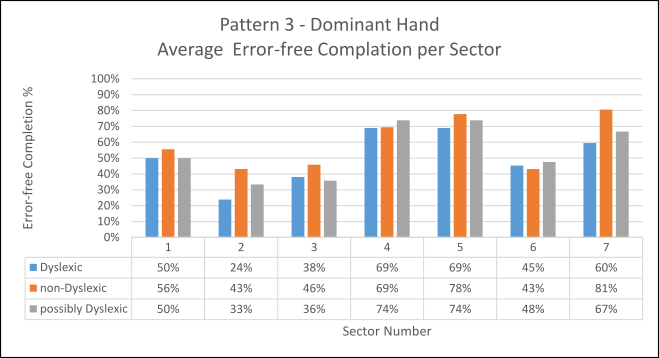
\includegraphics[width = \textwidth]{pat_3_com_dom}
			\caption{Pattern 3 - Average sector completion rate with no errors, executed with the dominant hand.}
			\label{fig_pat_3_com_dom}
		\end{figure}		
		
		\begin{figure}[!h]
			\centering
			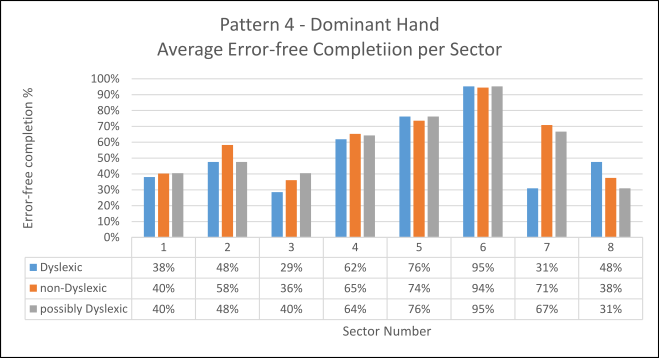
\includegraphics[width = \textwidth]{pat_4_com_dom}
			\caption{Pattern 4 - Average sector completion rate with no errors, executed with the dominant hand.}
			\label{fig_pat_4_com_dom}
		\end{figure}	
		
		A potential cause for the high error rate in these sectors may be due to the angle required to draw the line. However, this hypothesis is also somewhat unlikely due the fact that sectors of similar angles are also present in the patterns that do not share the same inconsistencies in error rate. 
		
		It is possible that the increase in error rate is related to the angle of previous movement. It appears that there is a higher error rate in sectors where there is a drastic change in angle from the previous sector. This is exemplified in pattern 4, where sectors 4, 5, and 6 form a gentle curve, followed by the steep angle of sector 7.
		
	\subsection{Analysis Summary}
		The analysis of results indicates that Fitts’s Law analysis of Dot-to-Dot Task results will not provide any meaningful data in regards to differentiation of Dyslexic and non-Dyslexic task participants. While Fitts’s Law may not appear to be an appropriate metric for Dyslexia detection, the analysis process revealed that the amount of errors made by Dyslexic task participants was noticeably larger the non-Dyslexic participants, suggesting that error rate analysis may be a more accurate alternative to Fitts’s Law for the analysis of Dot-to-Dot task results. Unfortunately it was not possible to further investigate the error rate of task participants, due to the limited number of patterns available for the Dot-to-Dot Task. Had error-analysis been considered as a metric during the initial planning stages of the project, a more concise and dedicated effort would have been made to properly collect and analyse the errors committed by task participants.	
\newpage